\chapter{Influence of fluid dynamics of the system on the extracted power}

\section{Introduction}

This chapter contains the results and discussion relating to the third objective of this thesis. As discussed in chapter \ref{chap:lit-review} the induced force $F_y$ of the system is mainly controlled by the behaviour of the top and bottom of the shear layer behaviour of the system. The current published work shows that the afterbody of the system has a significant influence on the galloping response \citep{Luo1994}. In this chapter, the influence of shear layer behaviour and hence, the influence of the afterbody on mean extracted power is explored.

Here, the influence of shear layer and it's reattachment on the mean power is studied by introducing a cross section which is a hybrid of a square and a triangle. The cross section is transformed gradually by manipulating the ratio of two length scales as shown in figure \ref{fig:hybrid_section}.

The stationary forcing data is presented for each cross section followed by the QSS power curves. Based on the QSS power data, an optimum cross section for power extraction is identified. Next, the underpinning reason for the negative regions of certain $C_y$ curves is discussed through surface pressure and flow velocity data. Following this, a comparison is made between QSS and DNS mean power at the optimum power cross section.       

A final summary is presented explaining the influence of the behaviour of the shear layer on mean power output and the preliminary design considerations to optimise the fluid mechanics to obtain an optimum power output. 


\section{Influence of the shear layers}

As highlighted in section \ref{subsec:fluid_mechanics_of_galloping} the afterbody of the cross section has a significant influence on galloping. This is because of the shear layer need to interact with the afterbody after separation at the leading edge. 


The $C_y$ vs $\theta$ curve increases till it reaches a maximum and then reduces as the induce angle is increased. The maximum of the induced lift occurs when the separated  shear layer (at the leading edge) closer to the surface of the body reattaches at the trailing edge \citep{Luo1994,Luo2003}. Therefore, by delaying the reattachment, the point where the maximum lift occurs can be shifted towards a higher induced angle which in the oscillatory case becomes a higher induced velocity. As shown in equation \ref{eqn:power_alt}, higher velocity is one factor that leads to higher power output. In order to test this hypothesis the shear layer reattachment was reduced by gradually tapering off the top and bottom sides of the square cross section trailing edges as sown in figure \ref{fig:hybrid_section}. The $\ratio$ was changed gradually from 1 to zero at increments of 0.25 where 1 being the square cross section and 0 being an isosceles triangle.    

\begin{figure}[!h]
\setlength{\unitlength}{\textwidth}

  \begin{picture}(1,0.36)(0,0.74)
    
  \put(0.2,0.76){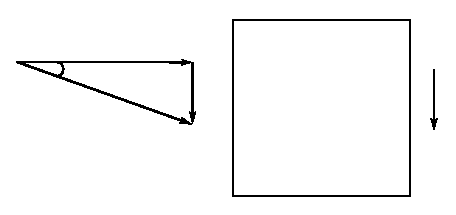
\includegraphics[width=0.5\unitlength]{./chapter-literature-revirw/fnp/setup-1.eps}}         
      
      
   
 	\put(0.315,1.04){$U$}
 	\put(0.3,0.95){$U_i$}
    \put(0.42,1.0){$\dot{y}$}
    \put(0.28,1.003){ $\theta$}
    \put(0.7,0.99){\small $(+)$}
      	

 	
 	 

     

  \end{picture}

 \caption{Induced angle of attack on a square prism due to the resultant of free-stream velocity of the fluid and transverse velocity of the body.}
    \label{fig:induced_lift_sketch}
\end{figure}

\section{Static body results}
 \label{sec:cross-sec-Static body results}
\begin{table}[ht]

\begin{center}
\setlength{\unitlength}{\textwidth}

\begin{tabular}{c c c c c} % centered columns (4 columns)
\hline\hline %inserts double horizontal lines
\\[0.2ex]
$\ratio$ & $a_1$ & $a_3$ & $a_5$ & $a_7$ \\ [0.8ex] % inserts table 
%heading
\hline 

\\[0.8ex]% inserts single horizontal line
$0$ &  -2.30617 & -269.075 & -59.2929 & 4.74389\\[0.8ex]
    & -5.08342 & -56.5390e & -160.505e & -105.773\\[0.8ex]
    &  4.40685 & 19.9213 & 22.8894 & 7.68556\\[1ex]


\\[0.8ex]% inserts single horizontal line
$0.25$ & -0.605146 & -19.4346 &-82.4463 & -94.4226\\[0.8ex]
      & 2.50538 & 9.91021  & 10.2712 & 3.94112 \\[1ex]

 \\[0.8ex]% inserting body of the table


 $0.5$ & 1.44734 & 4.83885  & -166.900e & -983.072 \\[0.8ex]% inserting body of the table
  & 1.51455e & 15.8476 & 52.5465 & 62.8067 \\ [1ex] % [1ex] adds vertical space
  
  \\[0.8ex]% inserting body of the table
  
   $0.75$ & 1.76938 & 35.2630 & -345.562 & -10072.7 \\[0.8ex]
          & 1.77553 & 43.0120 & 262.983 & 638.484 \\ [1ex]
          
          
  
  
\hline %inserts single line


\end{tabular}

\caption{Coefficient values used in the 7th order interpolation polynomial at $Re=200$. Data present for $\ratio=0-0.75$ at increments of $0.5$. Multiples polynomials were used to attain a better fit. The plot of the compound fit is presented in figure \ref{fig:lift_curves-hybrid}.} 
 
\label{table:cy-coefficients-hybrid} % is used to refer this table in the text
\end{center}
\end{table}



Stationary $C_y$ results were obtained for cross sections where $\ratio=1,0.75,0.5,0.25,0$ using DNS. Where $\ratio=1$ being the square and $\ratio=0$ being an isosceles  triangle. Table \ref{table:cy-coefficients-hybrid} shows the coefficients of the $7^{th}$ order interpolation polynomial for each cross section. In order to achieve a better fit, piecewise interpolation using multiple $7th$ order polynomials were incorporated for a single cross section. During the curve fitting process more importance was given for accurately fitting  the positive portion of the $C_{y}$ curve. This is because the power transfer from the fluid to the body occur in this region. 

\begin{figure}
  \setlength{\unitlength}{\textwidth}

  \begin{picture}(1,0.75)(0,0)
    % % %90
      % % % Parkinson Data 
      \put(0.035,0.5){\includegraphics[width=0.5\unitlength]{./chapter-cross-sections/fnp/lift_curve_sq.eps}}
      \put(0.495,0.5){\includegraphics[width=0.5\unitlength]{./chapter-cross-sections/fnp/lift_curve_075.eps}}
      \put(0.035,0.27){\includegraphics[width=0.5\unitlength]{./chapter-cross-sections/fnp/lift_curve_05.eps}}
      \put(0.495,0.27){\includegraphics[width=0.5\unitlength]{./chapter-cross-sections/fnp/lift_curve_025.eps}}
      \put(0.3,0.0){\includegraphics[width=0.5\unitlength]{./chapter-cross-sections/fnp/lift_curve_tri.eps}}
      
      
   
      
      
%      \put(0.23,0.00){ $\displaystyle\frac{c}{\rho\mathcal{A}U}$}
%      \put(0.73,0.00){ $\displaystyle\frac{c}{\rho\mathcal{A}U}$}

      \put(0.3,0.26){$\theta$}
      \put(0.76,0.26){$\theta$}
      \put(0.56,-0.01){$\theta$}
      
      \put(0.01,0.405){$\displaystyle C_y$}
       \put(0.01,0.65){$\displaystyle C_y$}
      \put(0.3,0.14){$\displaystyle C_y$}
      
      \put(0.106,0.705){\small(a)}
      \put(0.565,0.705){\small(b)}
      \put(0.106,0.475){\small(c)}
      \put(0.565,0.475){\small(d)}
      \put(0.37,0.207){\small(e)}
      

  \end{picture}

  \caption{Induced lift coefficient $C_y$ at different angles for selected cross sections. Data presented for cross sections, (a) square, (b) $\ratio=0.75$, (c) $\ratio=0.5$, (d) $\ratio=0.25$ and (e) triangle.}
  \label{fig:lift_curves-hybrid}
\end{figure}

The $C_y$ vs. $\theta$ curves in figure \ref{fig:lift_curves-hybrid} shows that the peak value of \cy\ shifts to the right as $\ratio$ is increased. These data agree with \citep{Luo1994} where the peak of the maximum \cy\ value was shifted to higher induced angles when reattachment was delayed. As $\theta$ is proportional to the transverse velocity of the body $tan{\theta}=\frac{\dot{y}}{U}$, it is clear that the maximum \cy\ would occur at higher induced velocities as \ratio\ is decreased between $0.25\leq\ratio<0.5$. Another interesting observation is that the presence of a negative portion prior to the point of maximum \cy\ in the \cy\ vs. $\theta$ curves as \ratio\ is decreased. In this region, \cy\ decreases reaches a minimum and then increases as $\theta$ is increased. The absolute value of the maximum is grater than the absolute value of the minimum. This negative portion starts to emerge at $\ratio=0.25$. However, the maximum value of \cy\ increases as \ratio\ is decreased providing an indication of a possibility of attaining a higher power output for cases with \ratio.

Yet, it is to be noted that the presence of the negative portion of the lift curve will oppose the motion of the body where the velocity of the body and the driving force will be out of phase. This will lead to an energy transfer from the body to the fluid and this power transfer which is in an unfavourable direction will result in  a reduction in mean power output.

 \section{QSS predictions}
  \label{sec:cross-sec-QSS}
  
 \subsection{Mean power output}
 \label{subsec:cross-sec-qss-mean power}
 
% !TeX spellcheck = en_GB
\begin{figure}[!htb]
  \setlength{\unitlength}{\textwidth}

        \begin{picture}(1,0.4)(-0.02,0)

 
      
      \put(0.08,0.02){\includegraphics[width=0.75\unitlength]{./FnP/mean_power_hyb.eps}}

      \put(0.46,0.00){\massdamp}
      
      
     
       \put(0.03,0.235){$\displaystyle\frac{P_{m}}{\rho \mathcal{A}U^3 }$}
      

      %\put(0.095,0.218){\small(a)}
      %\put(0.565,0.218){\small(b)}
      
    \end{picture}

  \caption{Dimensionless mean power obtained using QSS model as a function of \massdamp. Data presented for five selected cross sections, square ($\triangle$), $\ratio=0.75$ (+), $\ratio=0.5$ (\ding{117}), $\ratio=0.25$ ($\times$) and triangle (\ding{108}) at $\reynoldsnumber=200$, $\massstiff=100$.}
    \label{fig:power_curves}
\end{figure}

 %vspace{10cm}

 
Figure \ref{fig:power_curves} shows the mean power \massdamp\ vs. mean power for different cross sections namely $\ratio=1,0.75,0.5,0.25 \text{and} 0$. The maximum point of the \cy\ vs. $\theta$ represents the point of hear layer reattachment \citep{Luo1994}. It is discussed in \ref{sec:cross-sec-Static body results} that the maximum \cy\ occurs at higher induced angles as \ratio\ is decreased.Thus it can be concluded that the shear layer reattachment is delayed as \ratio\ is decreased. The mean power increases as \ratio\ is decrease where a significant increase in the maximum power could be observed. This meets the expectations where it was hypothesised that the mean power would increase as the shear layer re-attachment is delayed. A rapid increase in mean power could be observed below $\ratio\leq0.5$. This correspond with the large peak value of \cy\ which occur at a higher angle of attack which both contribute to a grater instantaneous power transfer. 

As $\ratio$  decreases beyond $\ratio\leq0.25$, as the mean power reaches the maximum a sudden drop could be observed as \massdamp\ is increased (eg. $\massdamp=0.39$ for $\ratio=0.25$). One interesting fact which could be observed is that the maximum power at $\ratio=0.25$ is larger that $\ratio=0$. This is against the expected outcome as the hypothesis was that by delaying the shear layer reattachment a higher mean power output could be gained.

As discussed in section \ref{sec:cross-sec-Static body results} the negative portion of the $C_y$ curve causes a reduction in maximum power at $\ratio=0$ in comparison with $\ratio=0.25$. Comparing  the initial negative portion of the $\cy$ vs $\theta$ plot of $\ratio=0.25$ and $\ratio=0$ cross section, it is clear that the area of the initial negative region is high in $\ratio=0$ which effectively transfers large amount of energy from the body to the fluid and therefore resulting a low power output.  


\subsection{Surface pressure}
  \label{subsec:cross-sec-surface pressure}
  

In order to investigate further the cause of this negative region, surface pressure data of static DNS simulations were analysed for the isosceles triangle ($\ratio=0$) at $\theta=4^{\circ}$, $\theta=16^{\circ}$ and $\theta=21^{\circ}$. These points correspond to a negative \cy\ that is further decreasing which increasing $\theta$, a negative \cy\ that is increasing with increasing $\theta$ and a significantly positive value of \cy.   
  
\begin{figure}
  \setlength{\unitlength}{\textwidth}

        \begin{picture}(1,1.1)(0,0.35)

      % % % Parkinson Data 
      \put(0.1,1.1){\includegraphics[width=0.75\unitlength]{./chapter-cross-sections/fnp/surf-pres-tri-4.eps}}
      \put(0.1,0.737){\includegraphics[width=0.75\unitlength]{./chapter-cross-sections/fnp/surf-pres-tri-16.eps}}
      \put(0.1,0.38){\includegraphics[width=0.75\unitlength]{./chapter-cross-sections/fnp/surf-pres-tri-21.eps}}
     
      
      



%      
    \put(0.21,1.41){\small(a)}
     \put(0.21,1.05){\small(b)}
     \put(0.21,0.69){\small(c)}
\put(0.1,0.95){$\displaystyle P_{s}$}
\put(0.1,1.3){$\displaystyle P_{s}$}
\put(0.1,0.56){$\displaystyle P_{s}$}
\put(0.26,0.35){Relative destance from the leading edge}

      
    \end{picture}

    \caption{Surface pressure of top (\ding{83}) and bottom (\ding{117})  surfaces of the static triangular cross section at (a) $\theta=4^\circ$, (b) $\theta=16^\circ$ \ and (c) $\theta=21^\circ$ A clear pressure difference is visible between the surfaces. The top surface comparatively has more negative pressure where a lift is created which results in a negative $C_y$ at $4^\circ$ and reduces as $\theta$ \ is increased, while the vice versa occurs at the top surface.}
    \label{fig:surf_pres}
\end{figure}

 %vspace{10cm}


Figure \ref{fig:surf_pres} shows the surface pressure of the top and bottom surfaces of the body ($\ratio=0$) starting from  the leading edges. At $\theta=4^{\circ}$, the pressure of the bottom of the body is grater than the top. Therefore, a pressure difference is created and a force is generated in the upward direction which according to the sign convention presented in \ref{fig:induced_lift_sketch}, is against the velocity of the body, hence giving a negative $\cy$. As $\theta$ (figure \ref{fig:surf_pres} (b)) is increased, to $16^{\circ}$ the gap between the surface pressure at the leading edge between the top and the bottom reduces. This effect results in the increase in $\cy$ (although it is still in the negative region). As $\theta$ is further increased at $21^{\circ}$ (figure \ref{fig:surf_pres} (c)) the surface pressure on the top side becomes grater than the bottom. Therefore, the net effect of the pressure difference is a positive $\cy$ which the driving force $F_y$ is in phase with the velocity of the body. 

\subsection{Velocity profiles at the points of flow separation}

Having established that the cause of the initial negative region of the $\cy$ vs. $\theta$ plot was the pressure difference mainly at the leading edge of the top and bottom surfaces of the cross section, further investigation was carried out to study the case.
\begin{figure}[!htb]
\setlength{\unitlength}{\textwidth}

  \begin{picture}(1,0.38)(0,0.74)
    
  \put(0.32,0.76){\includegraphics[width=0.32\unitlength]{./chapter-cross-sections/fnp/tri-sketch.eps}}         
      
      
   
 %	\put(0.28,0.937){$\theta$}
 	%\put(0.52,0.74){$l$}
   

 	
 	 

     

  \end{picture}

 \caption{Illustration of the lines along which the flow velocity magnitudes have been extracted. The data have been extracted along a line starting from the separation points in the outward direction (shown with arrows) for the top and bottom surfaces.}
    \label{fig:tri-sketch}
\end{figure}

A key variable which directly relates to the fluid dynamic pressure is the velocity of the fluid. Although not strictly true in all cases of viscous flows, one should expect that a higher flow speed correspond with a lower pressure from basic fluid dynamic theory. Hence, analysis of the velocity at the edges of flow separation was performed to obtain a clear understanding about the cause of the pressure differences occurred.   


In order to obtain a clear picture of the behaviour of the velocity, time averaged velocity magnitude data were obtained along lines spreading outwards starting from the top and bottom edges of flow separation. A clear illustration of these lines are depicted in figure \ref{fig:tri-sketch} .The lengths of these lines were equal to the width of the cross section. Data were obtained for the same cases presented earlier i.e. isosceles triangle ($\ratio=0$) at $\theta=4^{\circ}$, $\theta=16^{\circ}$ and $\theta=21^{\circ}$.

\begin{figure}[!h]
  \setlength{\unitlength}{\textwidth}

        \begin{picture}(1,1.1)(0,0.35)

      % % % Parkinson Data 
      \put(0.1,1.1){\includegraphics[width=0.75\unitlength]{./chapter-cross-sections/fnp/vel_prof-tri-4.eps}}
      \put(0.1,0.737){\includegraphics[width=0.75\unitlength]{./chapter-cross-sections/fnp/vel_prof-tri-16.eps}}
      \put(0.1,0.38){\includegraphics[width=0.75\unitlength]{./chapter-cross-sections/fnp/vel_prof-tri-21.eps}}
     
      
      



%      
    \put(0.21,1.41){\small(a)}
     \put(0.21,1.05){\small(b)}
     \put(0.21,0.69){\small(c)}
\put(0.1,0.95){$\displaystyle V_m$}
\put(0.1,1.3){$\displaystyle V_m$}
\put(0.1,0.56){$\displaystyle V_m$}
\put(0.34,0.35){Distance from the leading edge}

      
    \end{picture}

    \caption{Velocity magnitudes of the flow along a line parallel to the front surface spreading towards top (\dashedrule) and bottom (\solidrule) boundaries (figure \ref{fig:tri-sketch}). These two lines (for the top and bottom surfaces) start from the top and bottom leading edges of the triangular cross section. Data present (a) $\alpha=4^\circ$, (b) $\alpha=16^\circ$ \ and (c) $\alpha=21^\circ$.}
    \label{fig:vel-profile}
\end{figure}

 %vspace{10cm}


The velocity profiles at the chosen three incident angles are presented in figure \ref{fig:vel-profile}. A sudden rise of velocity magnitude could be observed at the flow separation points. The velocity magnitude at the top separation point  at $\theta= 4^{0}$ (figure \ref{fig:vel-profile} (a)) is higher than the bottom separation point, leading to a lower pressure at the top edge. However, the velocity magnitude at the bottom edge becomes grater than the top edge at $\theta=16^{\circ}$. The difference between the top and bottom velocity magnitude at the separation points tends to increase as $\theta$ is increased to $21^{\circ}$, where the velocity magnitude at the bottom being grater than the top (figure \ref{fig:vel-profile} (c)). This effectively creates the pressure difference created in figure \ref{fig:surf_pres} (c), which leads to a positive \cy\ and results in a forcing which is in phase with the velocity of the body. It could be seen \cy\ is governed by two mechanisms. Initially at $\theta= 4^{0}$ fundamental fluid mechanics govern \cy\. It could be said that Bernoulli's theorem and continuity governs this region. The cross section profile behaves similarly to an aerofoil. Thus \cy\ is generated similar to the mechanics involved in generating lift of an aerofoil. However, as $\theta$ is increased from $\theta=16^{\circ}$ to $21^{\circ}$, the proximity of the shear layer to the wall of the body (explained in subsection \ref{subsec:c_y and shear layers}) starts to govern the behaviour of \cy\ and hence, creating the positive region of the \cy\ vs. $\theta$ curve. 


\section{Fluid-structure interaction (DNS) results}
\label{sec:cross-sec-FSI-results}

\subsection{Mean power data}
\label{subsec:cross-sec-dns-mean-power}

As discussed in section \ref{sec:chp-pi_1_pi2_dns} the main limitation of the QSS model is the assumption that the only driving force of the system is $F_{y}$ which is generated by the fluid dynamic forces at the induced velocity . However, it was proven that this is not the case as vortex shedding have a significant influence with other non-linear disturbances on mean power as \massstiff\ decreases. Nevertheless, it was also concluded that a good agreement for power could be made at high \massstiff\ for the square cross section. Therefore, a comparison study between QSS and DNS mean power was carried out on the different cross section at high \massstiff\ (i.e.$\massstiff=1000$). As it was evident from figure \ref{fig:power_curves} that the maximum power occur between $1<\ratio<0.25$, DNS mean power data were obtained between $0.25\leq\ratio\leq1$.   

Both  DNS and QSS mean power data figure \ref{fig:DNS-power} show that \ratio\ decreases maximum mean extracted power increases following a similar trend. Thus these results reinforce the hypothesis proposed earlier; specifically a higher mean power can be achieved by delaying the flow re-attachment. 

However, a significant error (calculated using equation \ref{eqn:error_calculation}) between QSS and DNS power could be observed as \ratio\ increased. The quantified errors presented in \ref{fig:error-hybrid} clearly shows the exponential increase in the $\%$ error as $\ratio \rightarrow 0.25$. The likely cause of this significant error could be due to the non-linear interactions and the presence of non-linear forcing other than the induced force $F_{y}$.

\begin{figure} [htb]
  \setlength{\unitlength}{\textwidth}

        \begin{picture}(1,0.46)(0,0.4)

      \put(0.1,0.45){\includegraphics[width=0.75\unitlength]{./chapter-cross-sections/fnp/qss-dns-mean-power.eps}}
      
%       \put(0.07,0.95){$\displaystyle\frac{V}{D}$}
%       \put(0.07,1.3){$\displaystyle\frac{A}{D}$}
       \put(0.06,0.68){$\displaystyle\frac{P_{m}}{\rho \mathcal{A}U^3 }$}
%       \put(0.5,0.4){$\massdamp$}
       \put(0.5,0.42){$\displaystyle\ratio$}
    
    \end{picture}

  % \caption{Comparison of maximum power between QSS and DNS data obtained using 3 point local quadratic curve fitting.The error was obtained using Eq:\ref{eqn:error_calculation}}
    \caption{Comparison of the maximum power obtained using DNS ($\displaystyle\bullet$) data and predicted by QSS ($\times$) model as a function of \ratio. Data obtained at $\massstiff=1000$ ($\mstar=201.3$) and $\reynoldsnumber=200$. Similar trends are present for both QSS and DNS data. A significant reduction in power could be observed as $\ratio \rightarrow 1$}
    \label{fig:DNS-power}
\end{figure}

 %vspace{10cm}
\begin{figure}
  \setlength{\unitlength}{\textwidth}

        \begin{picture}(1,0.4)(0,0.4)

      \put(0.1,0.45){\includegraphics[width=0.75\unitlength]{./chapter-cross-sections/fnp/qss-dns-pow-erroe.eps}}
      
%       \put(0.07,0.95){$\displaystyle\frac{V}{D}$}
%       \put(0.07,1.3){$\displaystyle\frac{A}{D}$}
       \put(0.08,0.58){\rotatebox{90}{\%   error}}
%       \put(0.5,0.4){$\massdamp$}
       \put(0.5,0.4){$\displaystyle\ratio$}
    \end{picture}

  % \caption{Comparison of maximum power between QSS and DNS data obtained using 3 point local quadratic curve fitting.The error was obtained using Eq:\ref{eqn:error_calculation}}
    \caption{The percentage error calculated using equation \ref{eqn:error_calculation} between the maximum power obtained using DNS data and predicted by QSS model as a function of \ratio. The error reduces significantly as $\ratio \rightarrow 1$}
    \label{fig:error-hybrid}
\end{figure}

 %vspace{10cm}
 
\subsection{Flow-filed data}
 
 In order to investigate further on the error between QSS and DNS results, flow-filed data were analysed on a. The chosen cross section to perform this task was $\ratio=0.25$ at $\massdamp=0.26$ which is the case where the maximum mean power could be obtained in among all cases simulated using DNS. 
 
% !TeX spellcheck = en_GB
\begin{figure}[!htb]
  \setlength{\unitlength}{\textwidth}

        \begin{picture}(1,0.4)(-0.02,0)

 
      
      \put(0.08,0.02){\includegraphics[width=0.75\unitlength]{./chapter-cross-sections/fnp/fsi_flow_sketch.eps}}

      %\put(0.46,0.00){\massdamp}
      
      
     
       %\put(0.03,0.235){$\displaystyle\frac{P_{m}}{\rho \mathcal{A}U^3 }$}
      

      %\put(0.095,0.218){\small(a)}
      %\put(0.565,0.218){\small(b)}
      
    \end{picture}

  \caption{}
    \label{fig:power_curves}
\end{figure}

 %vspace{10cm}


The time averaged flow-fields were obtained at 3 selected points of the velocity signal. These points were point 1 where $\dot{y}$ is maximum, point 2 where $\dot{y}$ close to zero and further decreasing and point 3 where $\dot{y}$ is close to zero but moving towards the positive direction. A depiction of these points are presented in figure \ref{fig:FSI_sketch}. The averaging was carried out over a vortex-shedding cycle, where the starting and end times were defined to evenly bracket the point in consideration to attain the average flow-filed at that point. Time averaged stationary flow-flow field data of the corresponding induced angles were also obtained for comparison.


\begin{figure}[!htb]
  \setlength{\unitlength}{\textwidth}

  \begin{picture}(1,1.2)(0,0)
    % % %90
      % % % Parkinson Data 
      \put(0.005,0.8){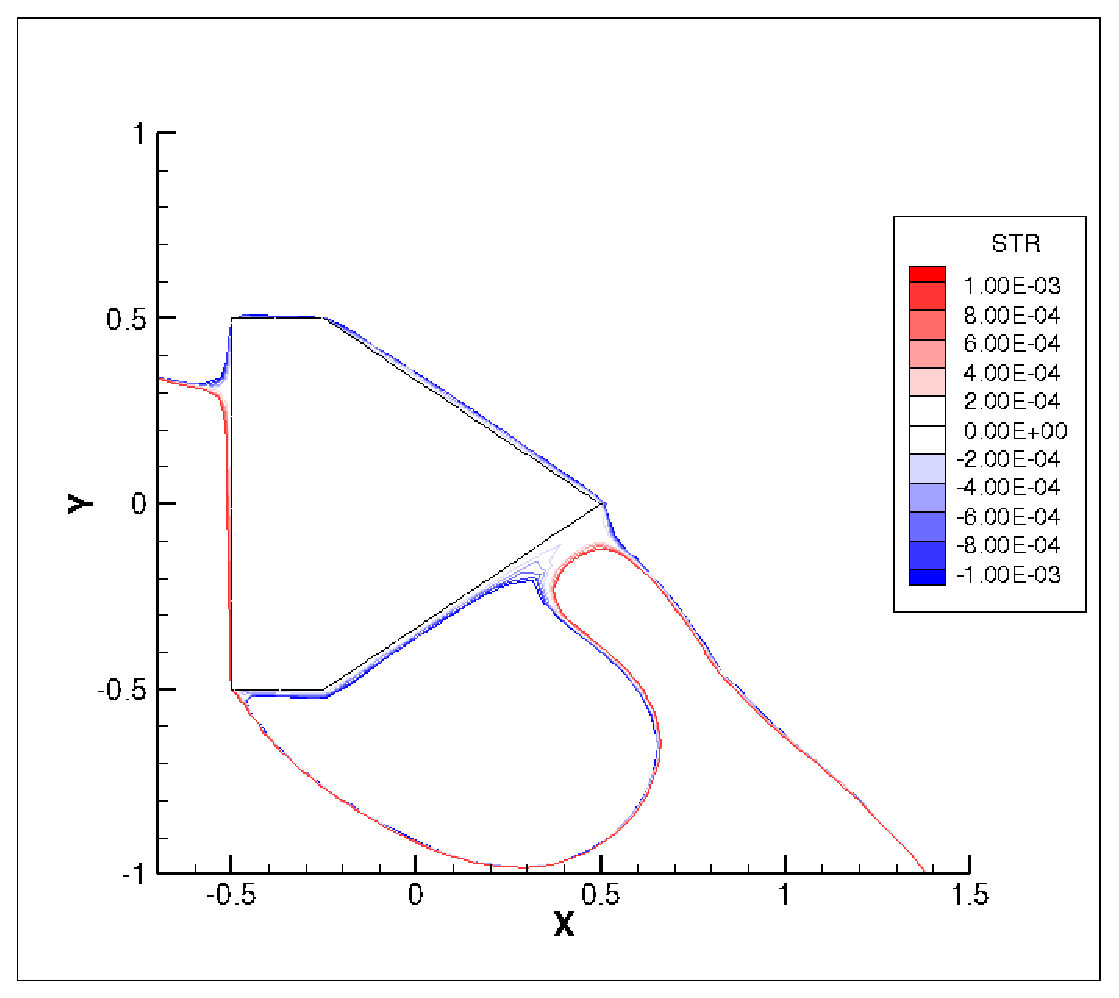
\includegraphics[width=0.4\unitlength]{./chapter-cross-sections/fnp/fsi-0.25-1.eps}}
      \put(0.005,0.4){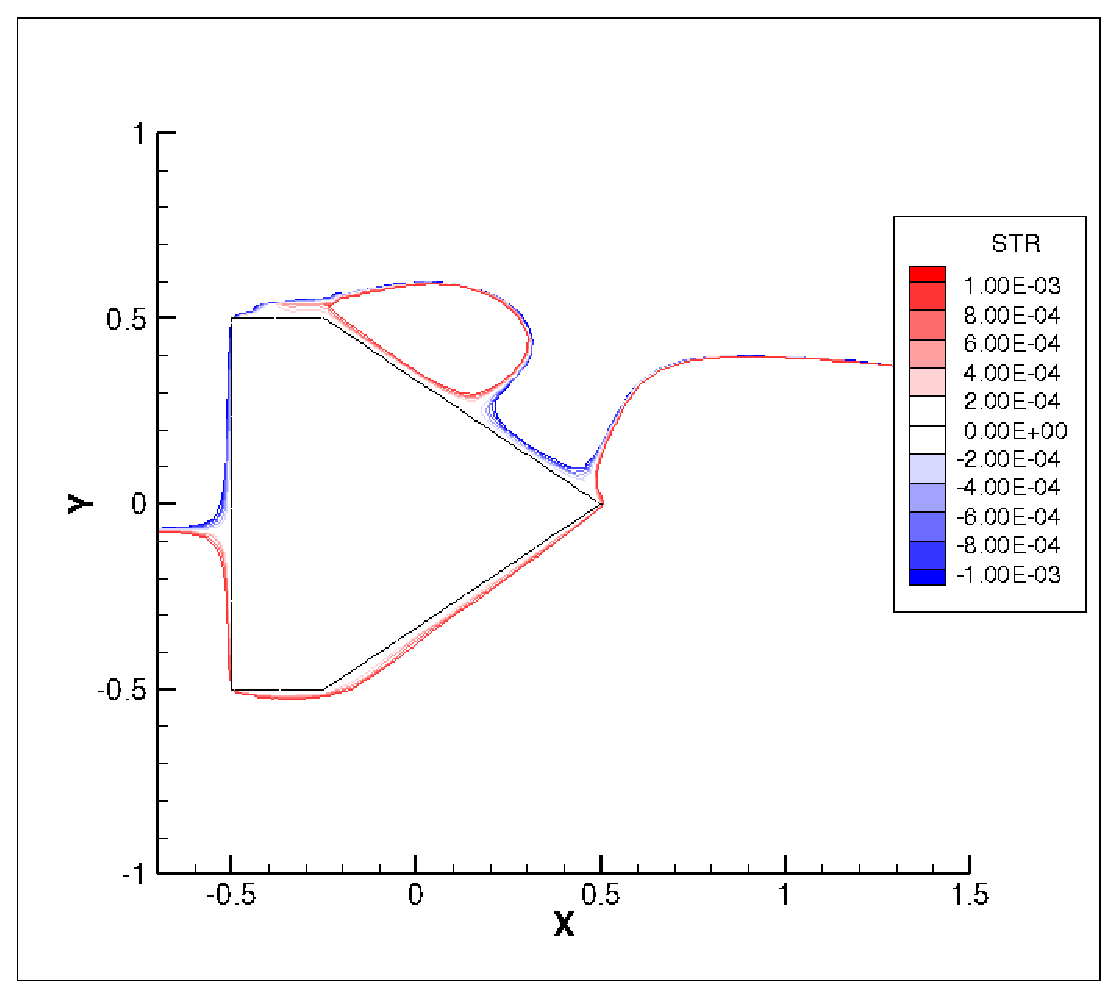
\includegraphics[width=0.4\unitlength]{./chapter-cross-sections/fnp/fsi-0.25-2.eps}}
      \put(0.005,0.0){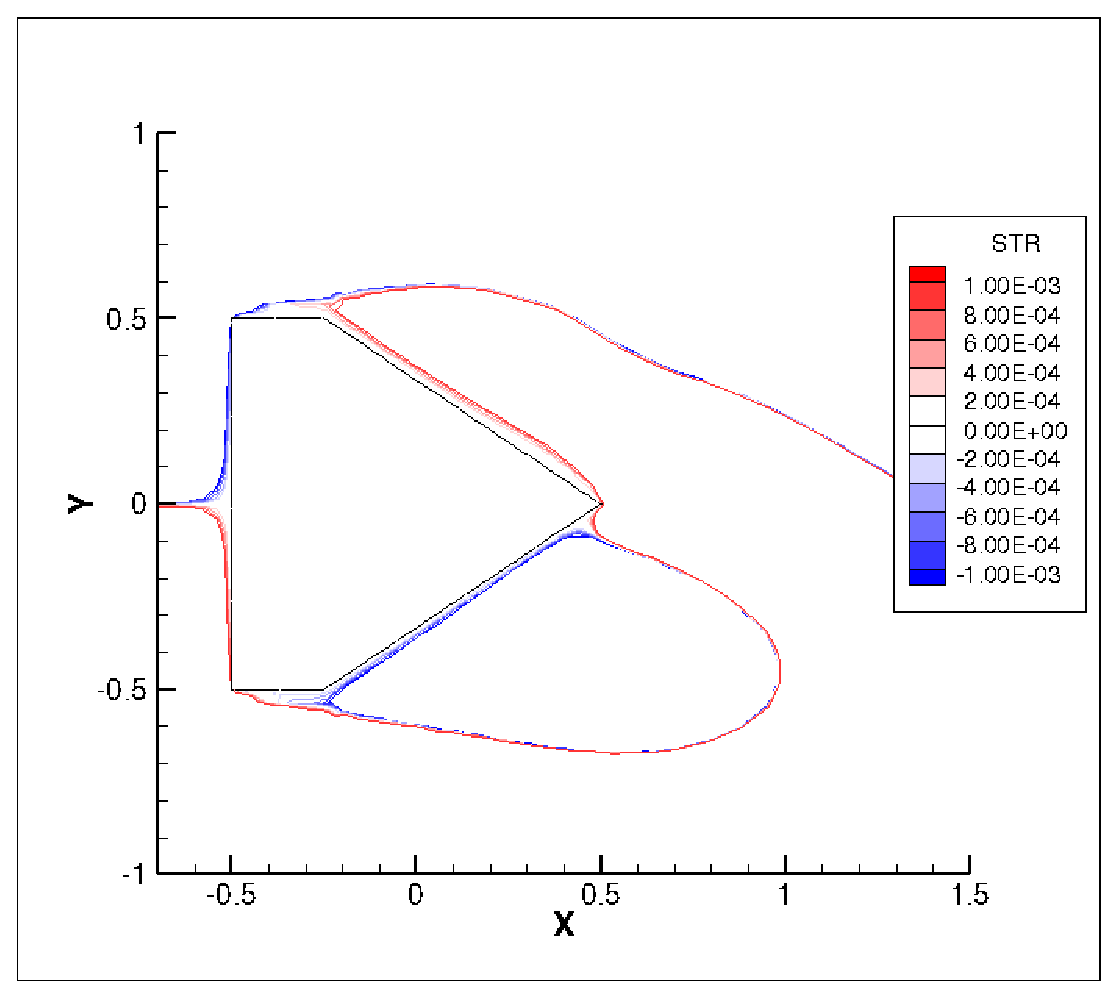
\includegraphics[width=0.4\unitlength]{./chapter-cross-sections/fnp/fsi-0.25-3.eps}}

      
      
      \put(0.505,0.8){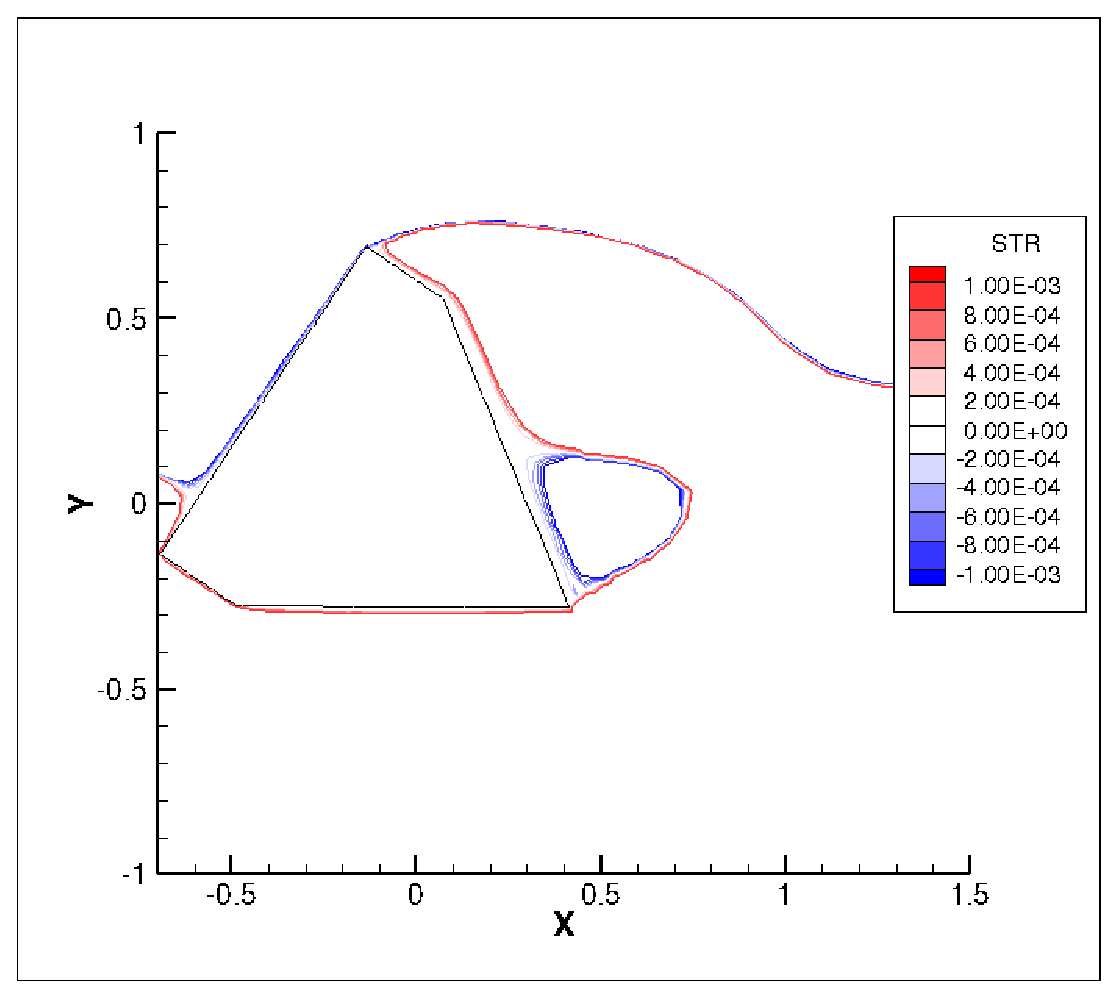
\includegraphics[width=0.4\unitlength]{./chapter-cross-sections/fnp/qss-0.25-1.eps}}
      \put(0.505,0.4){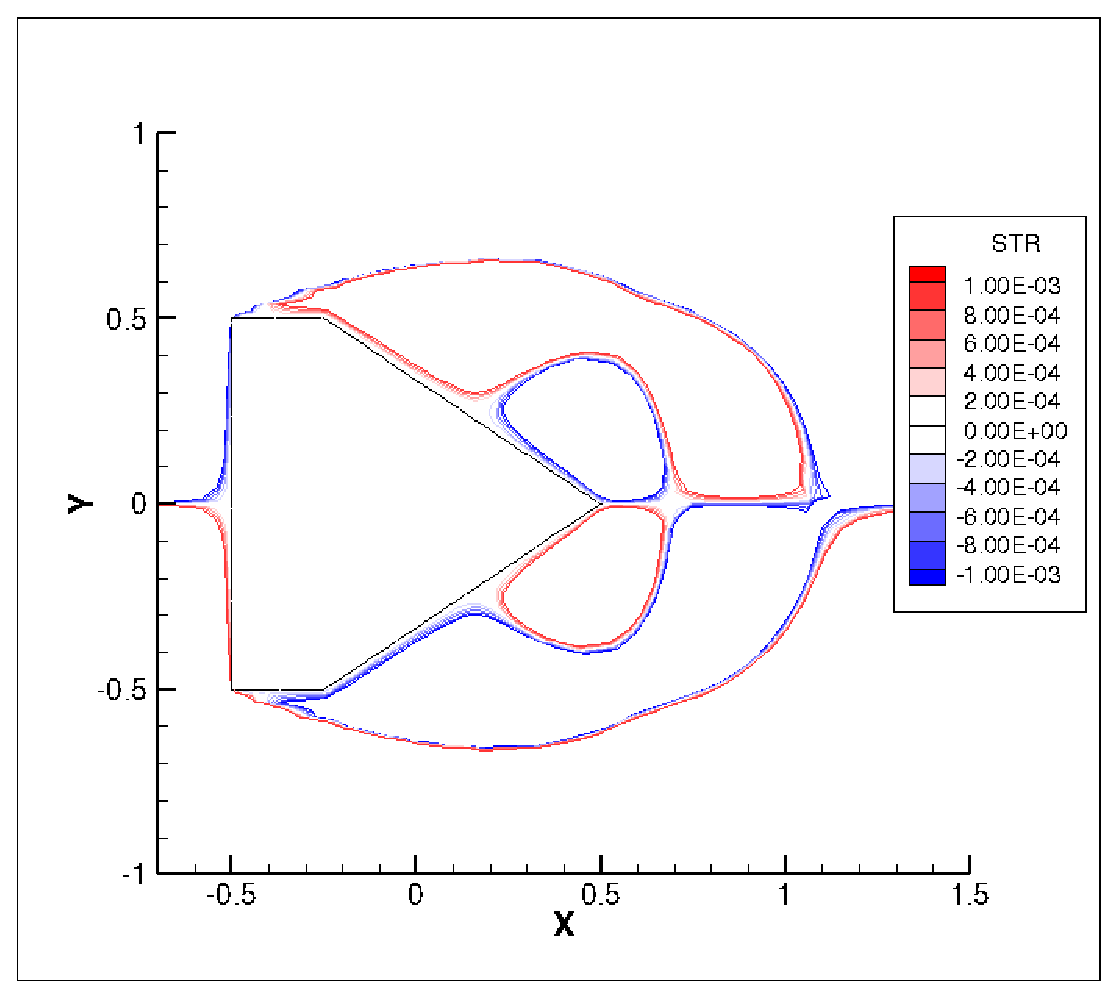
\includegraphics[width=0.4\unitlength]{./chapter-cross-sections/fnp/qss-0.25-3.eps}}
      \put(0.505,0.0){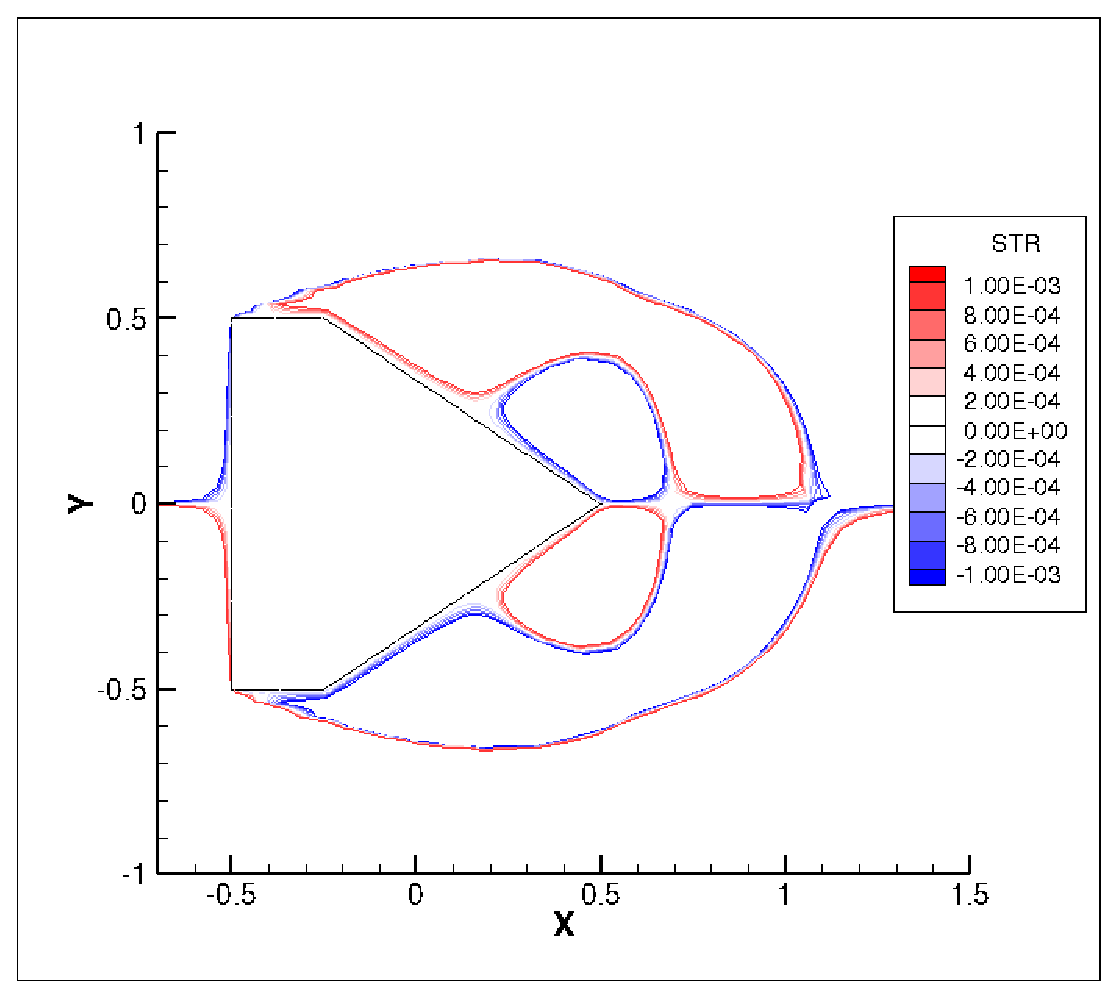
\includegraphics[width=0.4\unitlength]{./chapter-cross-sections/fnp/qss-0.25-3.eps}} 
      
      
%      \put(0.23,0.00){ $\displaystyle\frac{c}{\rho\mathcal{A}U}$}
%      \put(0.73,0.00){ $\displaystyle\frac{c}{\rho\mathcal{A}U}$}


      
      \put(0.01,1.125){\small(a)}
      \put(0.510,1.125){\small(b)}
      \put(0.01,0.725){\small(c)}
      \put(0.510,0.725){\small(d)}
      \put(0.01,0.33){\small(e)}
      \put(0.510,0.33){\small(f)}
      
   
   
      

  \end{picture}

  \caption{Time averaged stream functions of stationary and oscillating flow-fields of the hybrid cross section ($\ratio=0.25$), averaged over a vortex shedding cycle. (a), (c) and (e) the averaged stream functions of the oscillating case at $t=2295.763$ (point 1), $t=2305.897$ (point 2) and $t=2325.870$ (point 3) . (b), (d) and (f) are the stream functions of the flow field of the stationary body corresponding to the induced angles of (a), (c) and (e).}  
  \label{fig:flow_field_FSI}
\end{figure}

Figure \ref{fig:flow_field_FSI} shows the time averaged stream functions for points 1, 2 and 3 and the stationary time averaged flow-field data for the corresponding induced angles. Comparison between FSI and stationary data at point 1 (Figure \ref{fig:flow_field_FSI} (a) and (b)) shows a significant difference of the stream functions even at the leading edge.

In contrast, at point 2 and 3 the stream functions at the leading edge of the FSI simulations are similar to that of the stationary simulations. At point 2 both the FSI (figure \ref{fig:flow_field_FSI} (b)) and stationary (figure \ref{fig:flow_field_FSI} (c)) show similar flow behaviour until separation. A single circulation bubble at the top is formed in the FSI case where a symmetrical formation of circulation bubbles could be observed in the stationary case. A similar behaviour of the stream functions could be observed between point 3 for FSI (figure \ref{fig:flow_field_FSI} (d)) and stationary (figure \ref{fig:flow_field_FSI} (e)) cases. 

According to the assumptions of the QSS theory the flow-fields between the stationary and FSI cases at points 2 and 3 should be more or less identical as the induced velocities are zero therefore the induced angles are zero. However, the observations of the FSI case is significantly different. This indicates that there are significant non linear forcing is present as \ratio decreases which could be a result of the higher induced angles and therefore the higher velocities involved. 

Thus, one of the key conclusions could be gained is that the QSS predictions deviates significantly for mean power predictions as \ratio\ decreases. This is due to the fact that the forcing driving the system is not solely based on the induced velocity. Be that as it may the QSS model provides a reasonable predictions for power to obtain trends similar to DNS results. Therefore, QSS model could be used as a design and research tool to obtain preliminary data and conclusions to produce efficient galloping energy extraction systems. 

\section{Design considerations for a galloping energy extraction system through control of the fluid dynamics.}
\label{subsec:design-considerations-cross-section}
  
It is clear that delaying reattachment of the flow would lead to higher energy output. However, it is to be noted that even though a higher power output could be obtained by delaying separation, a region where the power is transferred from the body to the fluid will develop as \ratio\ is decreased. This can be observed through the negative region present in the $\cy$ curves beyond $\ratio<0.25$. As this negative region develops the maximum power which could be extracted reduces. This was observed in the power curves (figure \ref{subsec:cross-sec-qss-mean power}) where the maximum power of $\ratio=0$ was less than $\ratio=0.25$.

This fact leads to one important design consideration where the optimum cross section lies at the point where a balance of negative and positive regions could be obtained in the $\cy$ vs. $\theta$ curve. \citet{Barrero-Gil2010a} concluded that the first coefficient $a_1$ should satisfy  $a_1>0$ in order to obtain for good operation of an energy harvesting system. Here, it is explained more in detailed using the QSS model together with direct numerical simulations of FSI cases. 

As further consideration for future research, FSI and QSS work at $0<\ratio<0.25$ could be carried out to find the optimum ratio of $\ratio$ to obtain a maximum power output. Moreover, further work could be carried out investigate on the techniques to reduce the negative portion of the $\cy$ curve by applying modifications to the cross section. One such example could be rounding the corners of the cross section.

\section{Summary of Influence of fluid dynamics of the system on the extracted power} 
\label{sec:summary-diff-cross-sec}

The primary objective of the work presented in this chapter was to test the hypothesis whether higher power output could be obtained by delaying the flow reattachment. This was done by incrementally tapering off the top and bottom sides of the square cross section. A negative region in the $\cy$ vs. $\theta$ curve could be observed beyond $\ratio<0.25$. This region resulted in a power loss in a certain portion of the cycle as the driving force $F_y$ and the velocity $\dot{y}$ was out of phase.

The mean power vs. \massdamp\ curves showed an increase in maximum power as $\ratio$ was decreased until $\ratio=0.25$. At $\ratio=0$ the maximum power was less than $\ratio=0.25$. Further analysis of the \cy\ curve revealed that the negative region of $\ratio=0$ is grater than $\ratio=0.25$ hence, resulting in a lower maximum power output. 

Further investigations were carried out to find reasons for this negative region to exist. The surface pressure plots and the velocity magnitude profiles at the separation points revealed that this is due to the incidence angle and the cross section which resulted in changes in flow velocities at the separation points. 

Comparison with between the QSS maximum power data and the FSI data showed similar trends where the maximum power increased when \ratio\ was decreased proving that the hypothesis was correct. Be that as it may the error between the QSS and FSI simulation increased drastically as \ratio\ was reduced. Further investigations carried out using time averaged flow-filed data concluded that the mean flow of FSI simulations had significant deviations with the DNS stationary simulations carried out at corresponding induced angles. This was a result of the body moving towards higher induced angles and thereby moving towards higher velocities as \ratio\ was decreased. Therefore the primary assumption of QSS which is considering $F_y$ as the driving force of the system was no longer valid as other significant non-linear forcing was present in the system. Yet, the QSS model could be used as a tool to obtain initial approximations to design galloping energy harvesting systems as QSS data produced similar trends as the FSI simulations.

In order to obtain an efficient galloping one key design consideration is to obtain a cross section which has the optimum balance of the negative and positive regions of the $\cy$ vs. $\theta$ curve. Delaying the reattachment leads to higher power however as a consequence a negative region of $\cy$ emerges in \cy\ curve and therefore, transferring power from the body to the fluid. This region keeps on increasing between $0\leq\ratio\leq0.25$. Thus as a result an optimum \ratio should be obtained in order to get a balance between the negative and positive regions which leads to an efficient galloping energy harvesting system. 

As for future research and development, a further design consideration could be investigating the possibility of reducing the negative region of the \cy\ curve by making alterations to the cross section such as rounding the edges of flow separation. 

 

      




